% ============================================================
%  Appendix: Chapter 3 – Part 2 Supporting Information
%  Anti-breast cancer effects of carbon quantum dots:
%  in vivo angiogenesis and targeted arginase co-inhibition
% ============================================================

\appendix{Supporting Information for Chapter~3 (Part~2)}



% ------------------------------------------------------------
\section*{Experimental Procedures}
% ------------------------------------------------------------

\subsection*{X-Ray Diffraction}
Approximately 1\,g of powdered sample was placed in a sample holder of the XRD machine
and scanned at 0.1 step size; readings were recorded using a Co source
($K_{\alpha} = 1.79$\,\AA) at 25\,\textdegree C from $2\theta = 5^{\circ}$ to
$90^{\circ}$.

\subsection*{Measurement of Fluorescence Quantum Yield}
Powder samples were dispersed in distilled water (1\,mL) at room temperature
(25\,\textdegree C) and the sample absorbance was set to 0.1\,a.u.\ at the absorbance
maximum ($\lambda_{\max} = 325$\,nm). The absorption maximum was then used as the
excitation wavelength and the emission spectrum was recorded using a fluorescence
spectrophotometer. The relative quantum yield was calculated against coumarin as the
reference standard using Equation~\ref{eq:qy}:

\begin{equation}
  \phi_{f}^{i} = \frac{F_{i}\,f_{s}\,n_{i}^{2}}{F_{s}\,f_{i}\,n_{s}^{2}}\,\phi_{f}^{s}
  \label{eq:qy}
\end{equation}

\noindent where $\phi_{f}^{i}$ and $\phi_{f}^{s}$ are the photoluminescence quantum
yields of the sample and standard, respectively; $F_{i}$ and $F_{s}$ are the integrated
fluorescence intensities of the sample and reference; $f_{x} = 1 - 10^{-A_{x}}$ is the
absorption factor ($A$ is the absorbance of the solution); and $n_{i}$ and $n_{s}$ are
the refractive indices of the sample and reference, respectively.

\subsection*{Measurement of Acute Toxicity}
Six male mice of average body weight 25--30\,g were chosen and administered a limit dose
of 2\,g\,kg$^{-1}$ according to OECD guidelines for Acute Toxicity Test No.~425.
Briefly, a single oral dose (in distilled water) was administered and animals were
maintained for 28 days with standard diet. Body weight, behaviour, and mortality were
monitored throughout. Urine samples were analysed weekly using a urine-testing strip
(Urisign 10P, Recombigen Laboratories Pvt.\ Ltd.). All parameters are reported in
Table~\ref{tab:urine}. Sample size for all experiments was $n = 6$.

\subsection*{Hemocompatibility Test}
Rat RBCs were isolated from 3\,mL of whole blood by centrifugation
(4000\,rpm, 10--15\,min, 25\,\textdegree C) and washed three times with 0.1\,M PBS
(pH\,7.4). Washed RBCs ($1 \times 10^{6}$) were incubated with CQDs at concentrations
of 0.1, 0.2, 0.5, and 1.0\,mg\,mL$^{-1}$ for up to 8\,h. Following centrifugation
(4000\,rpm, 10--15\,min, 25\,\textdegree C), the supernatant was analysed at
$\lambda_{\max} = 570$\,nm (ELISA plate reader, BioTek Synergy H1). The pellet was
divided into two portions: (i) for osmotic fragility, RBCs were subjected to osmotic
stress in NaCl solutions ranging from 0.1\% to 1.0\% (w/v) for 15\,min followed by
absorbance measurement at 570\,nm; (ii) for morphological imaging, RBCs were stained
with Giemsa stain (5\,min), mounted on slides, and examined by light microscopy.

\subsection*{Platelet Agglomeration Assay}
Platelet-rich plasma (PRP) was isolated by centrifugation of citrated blood at
$100 \times g$ for 15\,min at room temperature. The straw-coloured supernatant was
collected, combined with nanoparticle solution or saline, and incubated at 37\,\textdegree C
for 30\,min. Turbidity indicating platelet agglomeration was assessed visually.

\subsection*{Platelet Adhesion Assay}
Fresh citrated PRP was incubated with nanoparticle solution for 30\,min at
37\,\textdegree C on clean, uncoated glass slides. Non-adherent cells were removed by
gentle PBS washing. Slides were air-dried, fixed in anhydrous methanol, and stained with
Wright--Giemsa stain for visualisation of adherent platelets under oil-immersion
microscopy (100$\times$).

\subsection*{Clot Retraction Assay}
PRP pre-incubated with CQDs for 30\,min was diluted 1:4 with saline. CaCl$_{2}$ solution
(150\,\textmu L, 200\,mM) was added to initiate clot formation. The clot was allowed to
retract at room temperature for 2\,h, after which images were captured and the volume of
expressed serum was measured.

\subsection*{Chick Embryo Irritation Assay}
Fertilised chicken eggs were incubated for 4 days with a window created as described in
the main text. UV-sterilised samples were inoculated on the yolk sac membrane and images
were acquired at 24\,h. PBS served as negative control, 1\% formaldehyde solution in PBS
(pH\,7.4) as positive control; all samples were diluted in PBS (pH\,7.4).

\subsection*{Hemolysis Study}
RBCs were obtained from fresh blood by centrifugation ($5000 \times g$, 10\,min) and
washed three times with PBS (pH\,7.4). RBCs were incubated with samples dissolved in
0.9\% saline at the indicated concentrations. Supernatant was collected at 30\,min, 1\,h,
2\,h, 4\,h, and 8\,h, and absorbance was measured at $\lambda_{\max} = 545$\,nm (BioTek
ELISA plate reader).

\subsection*{\textit{In Ovo} Developmental Toxicity Assay}
Fertilised chicken eggs were incubated for 36\,h and injected with 200\,\textmu L of
sample into the yolk. The hole was sealed with molten paraffin wax and incubation
continued for a further 48\,h. Uncontaminated embryos were collected, sacrificed by
cutting blood vessels, washed with PBS, and imaged through a stereo zoom microscope
equipped with crossed Polaroid filters to visualise internal and external structures.

\subsection*{ELISA}
Tissue lysates were prepared from tumour tissue collected from saline-treated and
CQD@250-treated mice. ELISA kits (Fine Test Chemicals, Invitrogen, and Elabscience
Bioinovation Inc.) were used according to manufacturer instructions to quantify TNF-$\alpha$,
IL-8, IL-1$\beta$, IL-6, IL-21, and T-cell markers.

% ------------------------------------------------------------
\section*{Supporting Figures}
% ------------------------------------------------------------

\begin{figure}[htbp]
  \centering
  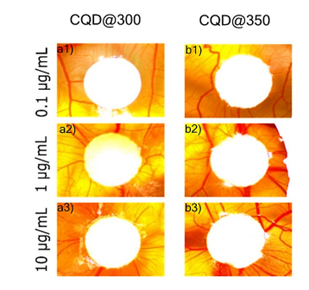
\includegraphics[width=0.55\textwidth]{appendix_figures/Picture9.png}
  \caption[UV--Vis absorbance spectra of CQD@250]{UV--Vis absorbance spectra of
    CQD@250 showing two broad bands at $\lambda_{\max} = 340$\,nm and 280\,nm.
    Inset shows emission under different excitation light sources. Spectra were
    acquired at varying concentrations (mg\,mL$^{-1}$) of CQD@250.}
  \label{fig:s1_uvvis}
\end{figure}

\begin{figure}[htbp]
  \centering
  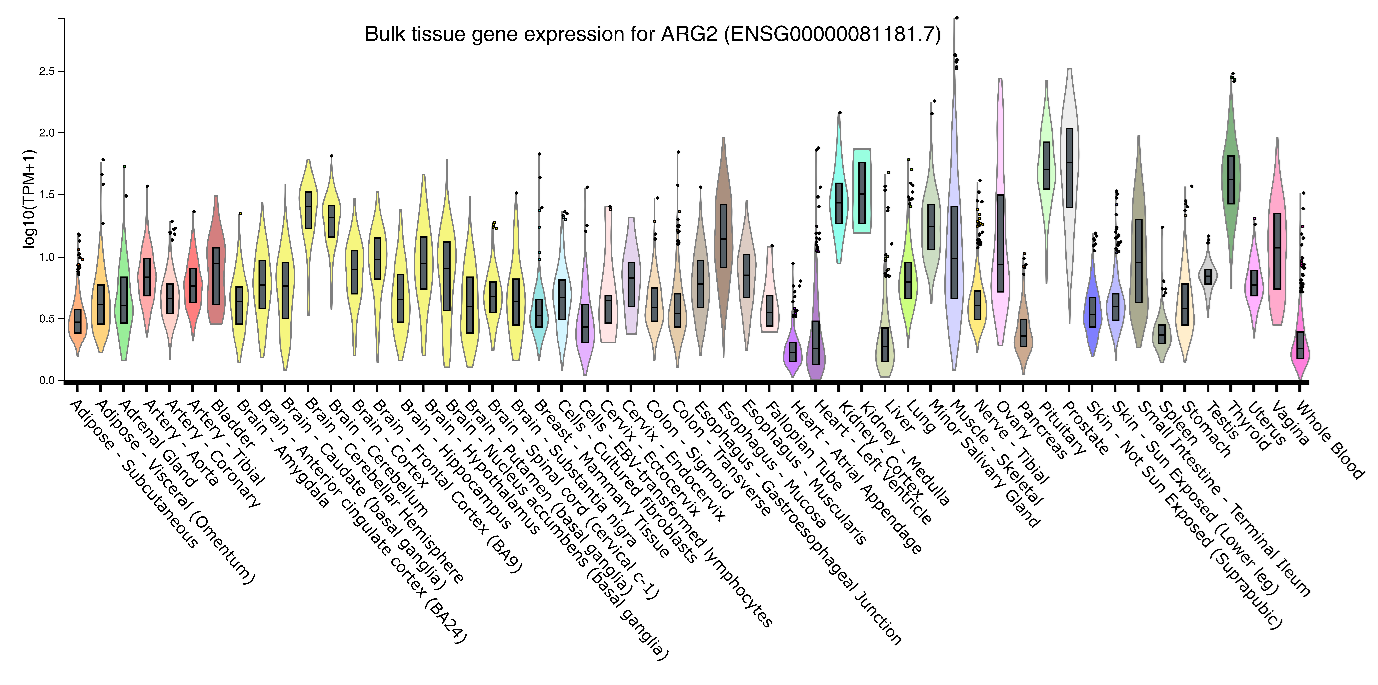
\includegraphics[width=0.75\textwidth]{appendix_figures/Picture3.png}
  \caption[Fluorescence spectroscopy of CQD@250]{Fluorescence spectroscopy analysis
    of CQD@250 (10\,\textmu g\,mL$^{-1}$, in water).
    \textbf{(a)}~Fluorescence emission spectrum (excitation at 325\,nm).
    \textbf{(b)}~Fluorescence lifetime decay profile.}
  \label{fig:s2_fl}
\end{figure}

\begin{figure}[htbp]
  \centering
  \begin{subfigure}[b]{0.9\textwidth}
    \includegraphics[width=\textwidth]{appendix_figures/Picture3_1.png}
    \caption{ARG1 (ENSG00000118520.14)}
  \end{subfigure}\\[8pt]
  \begin{subfigure}[b]{0.9\textwidth}
    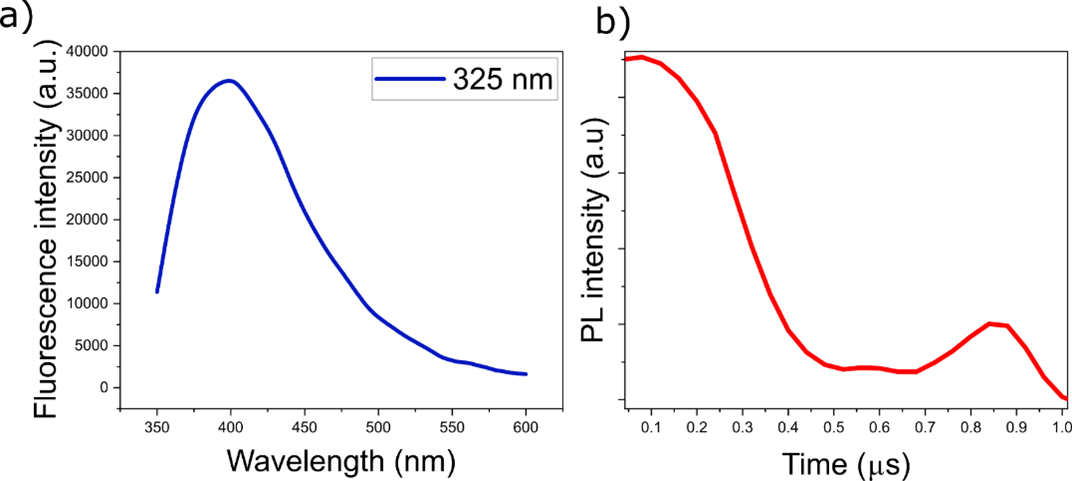
\includegraphics[width=\textwidth]{appendix_figures/Picture2.png}
    \caption{ARG2 (ENSG00000081181.7)}
  \end{subfigure}
  \caption[Bulk tissue gene expression of ARG1 and ARG2]{Bulk tissue gene expression
    profiles (log$_{10}$(TPM+1)) of \textbf{(a)}~ARG1 and \textbf{(b)}~ARG2 across
    human organs. Data obtained from the GTEx Portal (accessed 22 August 2024) and
    dbGaP accession phs000424.}
  \label{fig:s3_gtex}
\end{figure}

\begin{figure}[htbp]
  \centering
  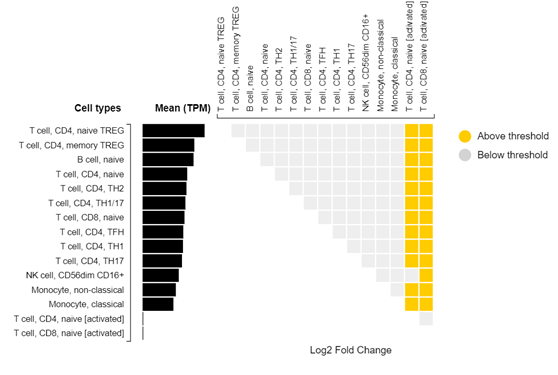
\includegraphics[width=0.85\textwidth]{appendix_figures/Picture6.png}
  \caption[Differential expression of ARG1 in immune cell subsets]{Differential
    expression of ARG1 in different immune cell subsets (DICE database). Threshold
    value of 3.1 indicates that ARG1 expression is highest in T-regulatory cells.}
  \label{fig:s4_dice}
\end{figure}

\begin{figure}[htbp]
  \centering
  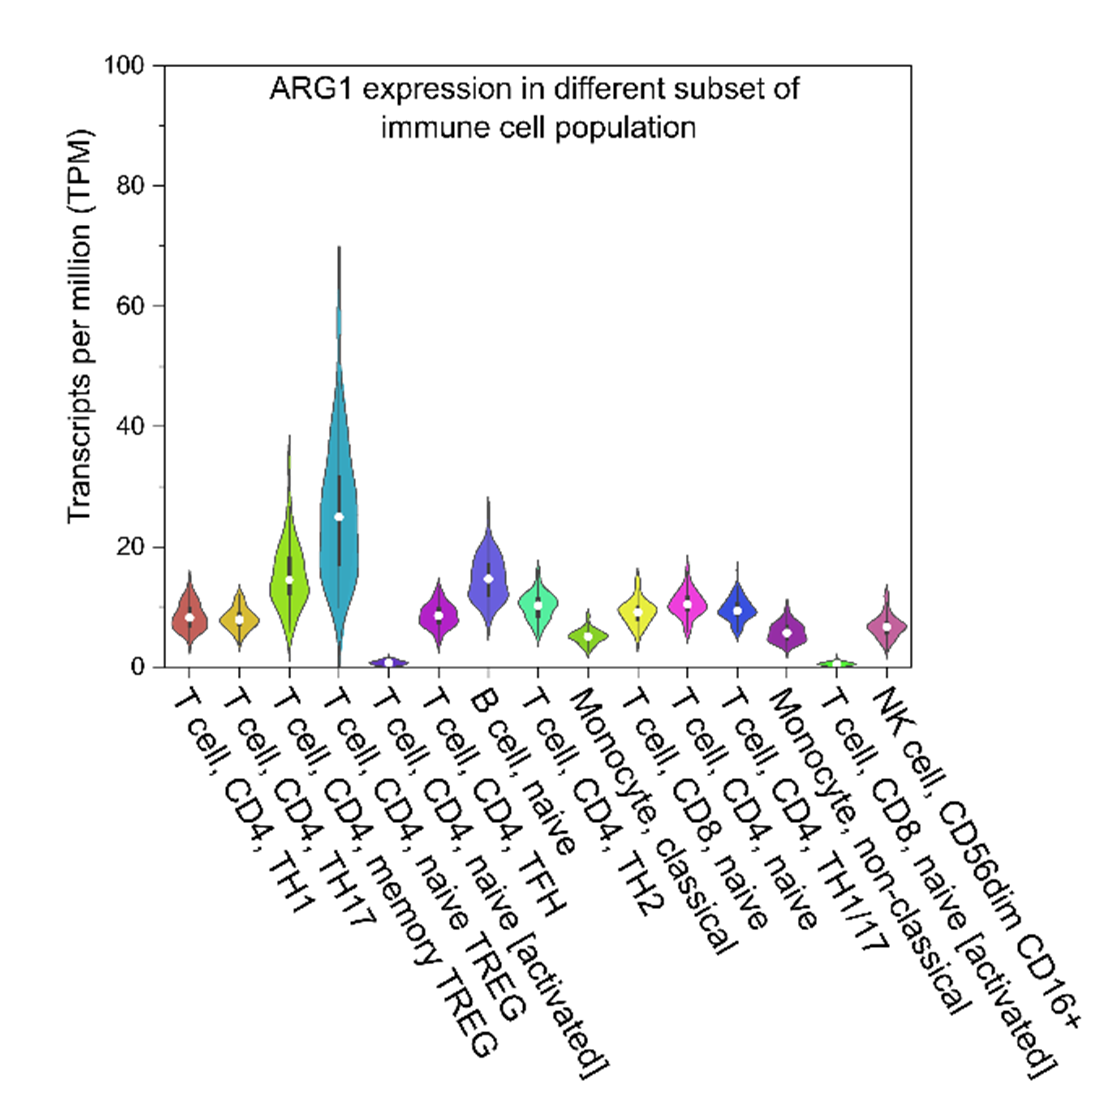
\includegraphics[width=0.55\textwidth]{appendix_figures/Picture7.png}
  \caption[scRNA-seq expression of ARG1 in immune cells]{Expression levels of ARG1
    in different immune cell populations based on single-cell RNA sequencing data
    from the DICE database.}
  \label{fig:s5_scrna}
\end{figure}

\begin{figure}[htbp]
  \centering
  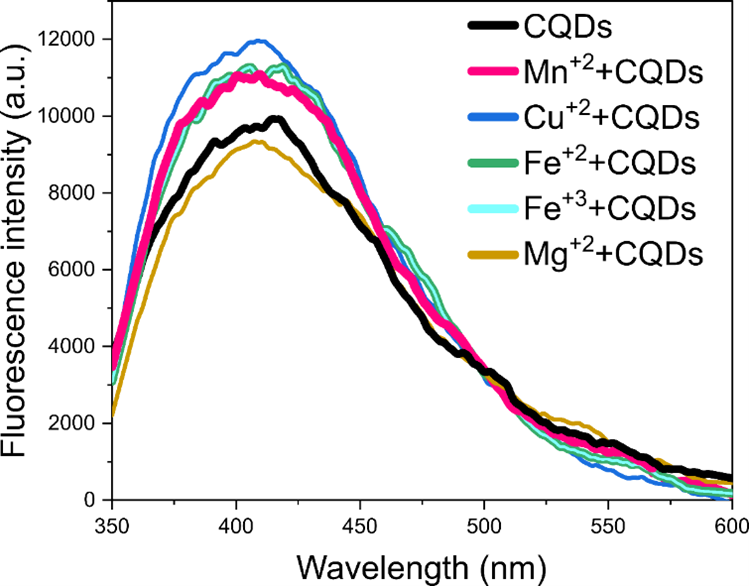
\includegraphics[width=0.65\textwidth]{appendix_figures/Picture20.png}
  \caption[Fluorescence of CQDs in presence of metal ions]{Change in fluorescence
    intensity of CQDs in the presence of different enzymatically active metal ions
    (Mn$^{2+}$, Cu$^{2+}$, Fe$^{2+}$, Fe$^{3+}$, Mg$^{2+}$) at excitation
    wavelength of 325\,nm.}
  \label{fig:s6_metal}
\end{figure}

\begin{figure}[htbp]
  \centering
  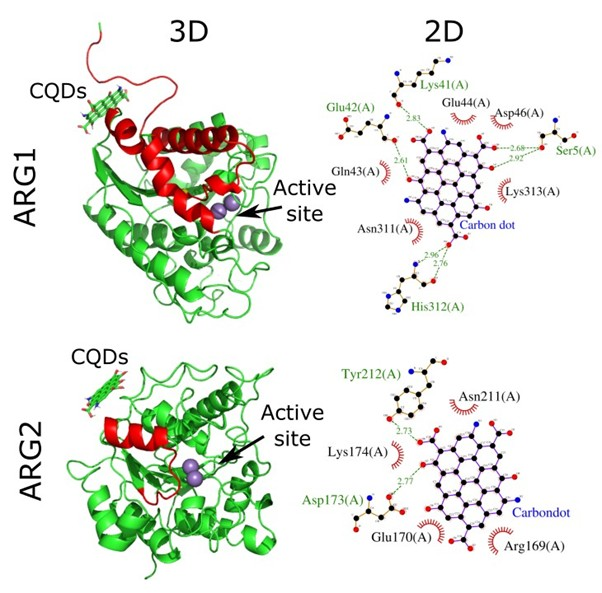
\includegraphics[width=0.65\textwidth]{appendix_figures/Picture15.jpg}
  \caption[CAM angiogenesis assay with CQD@300 and CQD@350]{Pictorial representation
    of the CAM angiogenesis assay. \textbf{(a1)}~0.1\,\textmu g\,mL$^{-1}$ CQD@300;
    \textbf{(a2)}~1\,\textmu g\,mL$^{-1}$ CQD@300;
    \textbf{(a3)}~10\,\textmu g\,mL$^{-1}$ CQD@300;
    \textbf{(b1)}~0.1\,\textmu g\,mL$^{-1}$ CQD@350;
    \textbf{(b2)}~1\,\textmu g\,mL$^{-1}$ CQD@350;
    \textbf{(b3)}~10\,\textmu g\,mL$^{-1}$ CQD@350.
    Cycle spoke-wheel pattern visible towards disk regions.}
  \label{fig:s7_cam}
\end{figure}

\begin{figure}[htbp]
  \centering
  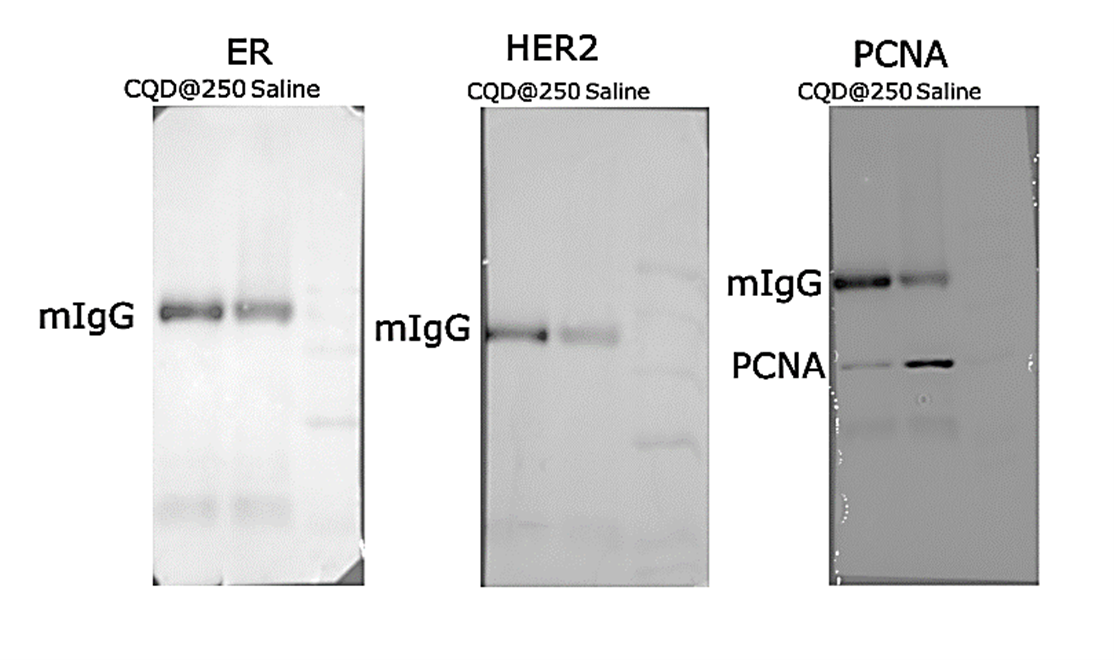
\includegraphics[width=0.80\textwidth]{appendix_figures/Picture10.png}
  \caption[Western blot analysis of ER, HER2, and PCNA]{Western blot analysis
    showing expression levels of oestrogen receptor (ER), HER2 (c-erbB-2, human
    epidermal receptor 2 analogue in mice), and PCNA (proliferating cell nuclear
    antigen) in CQD@250- and saline-treated groups. mIgG = mouse immunoglobulin G.}
  \label{fig:s8_wb}
\end{figure}

\begin{figure}[htbp]
  \centering
  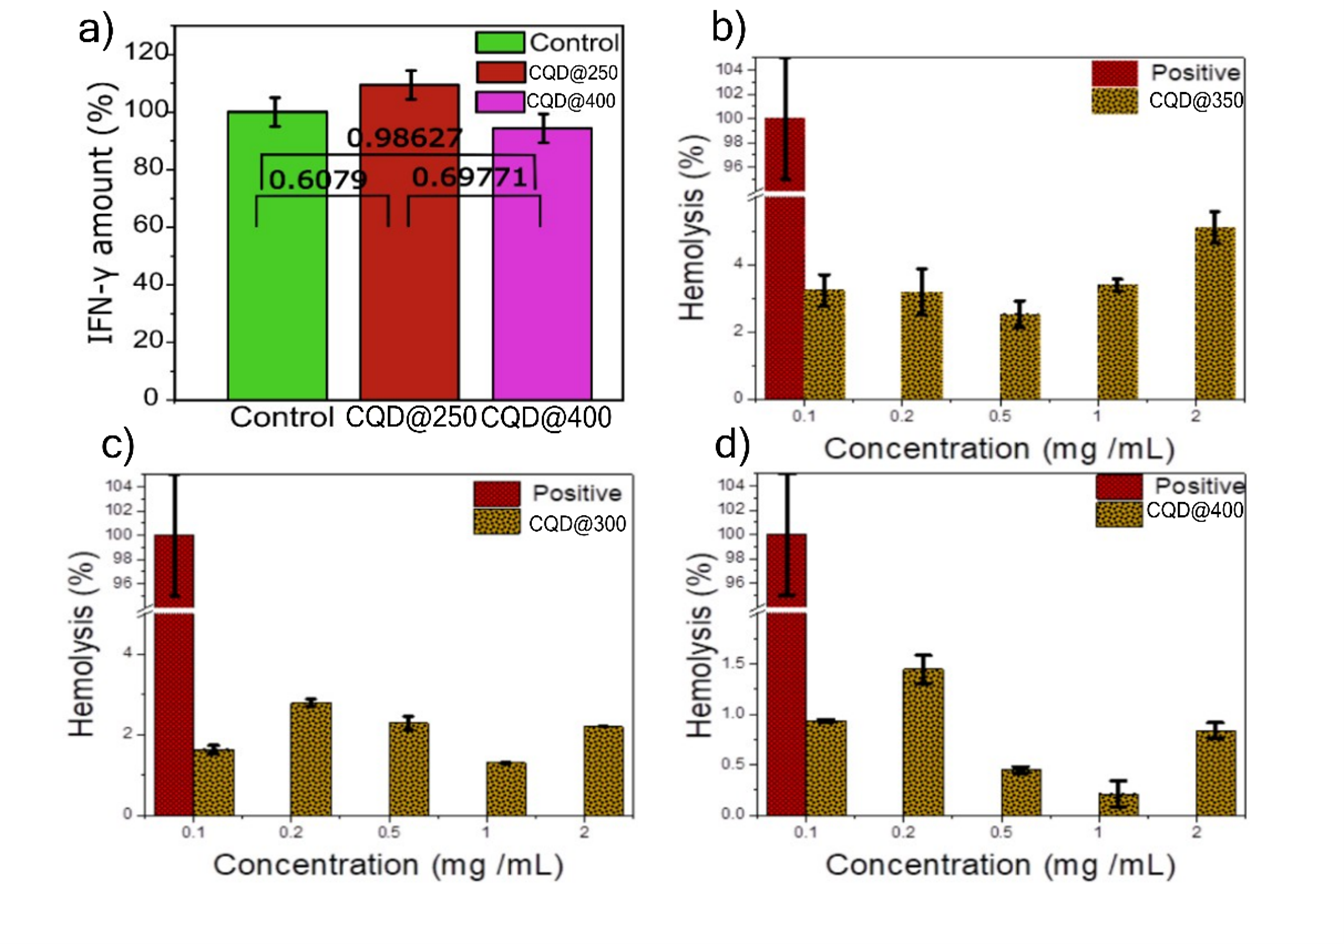
\includegraphics[width=0.85\textwidth]{appendix_figures/Picture11.png}
  \caption[IFN-$\gamma$ and hemolysis data for CQD variants]{
    \textbf{(a)}~IFN-$\gamma$ levels in the tumour microenvironment (Control,
    CQD@250, CQD@400; $p$-values shown).
    \textbf{(b)}~Hemolysis (\%) of RBCs treated with CQD@350.
    \textbf{(c)}~Hemolysis (\%) of RBCs treated with CQD@300.
    \textbf{(d)}~Hemolysis (\%) of RBCs treated with CQD@400.
    All data represent mean $\pm$ SD.}
  \label{fig:s9_ifn_hemo}
\end{figure}

\begin{figure}[htbp]
  \centering
  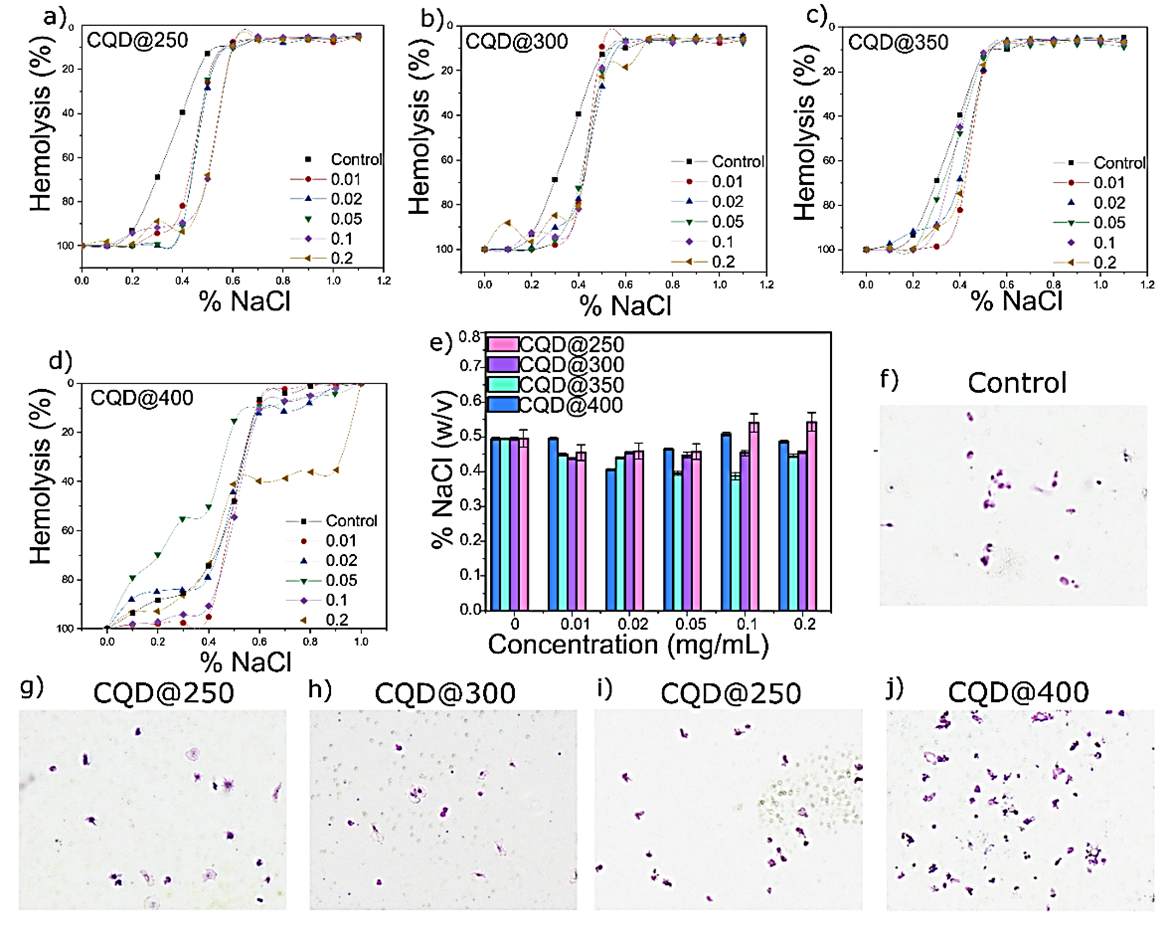
\includegraphics[width=\textwidth]{appendix_figures/Picture12.png}
  \caption[Hemocompatibility and platelet adhesion assay]{Hemocompatibility assay
    and platelet adhesion assay.
    Osmotic fragility of RBCs treated with
    \textbf{(a)}~CQD@250, \textbf{(b)}~CQD@300, \textbf{(c)}~CQD@350, and
    \textbf{(d)}~CQD@400 at varying concentrations.
    \textbf{(e)}~NaCl concentration at which 50\% hemolysis occurred for each sample.
    \textbf{(f)--(j)}~Platelet adhesion assay on clean, untreated glass surfaces after
    30\,min of treatment with different samples.}
  \label{fig:s10_hemo_platelet}
\end{figure}

\begin{figure}[htbp]
  \centering
  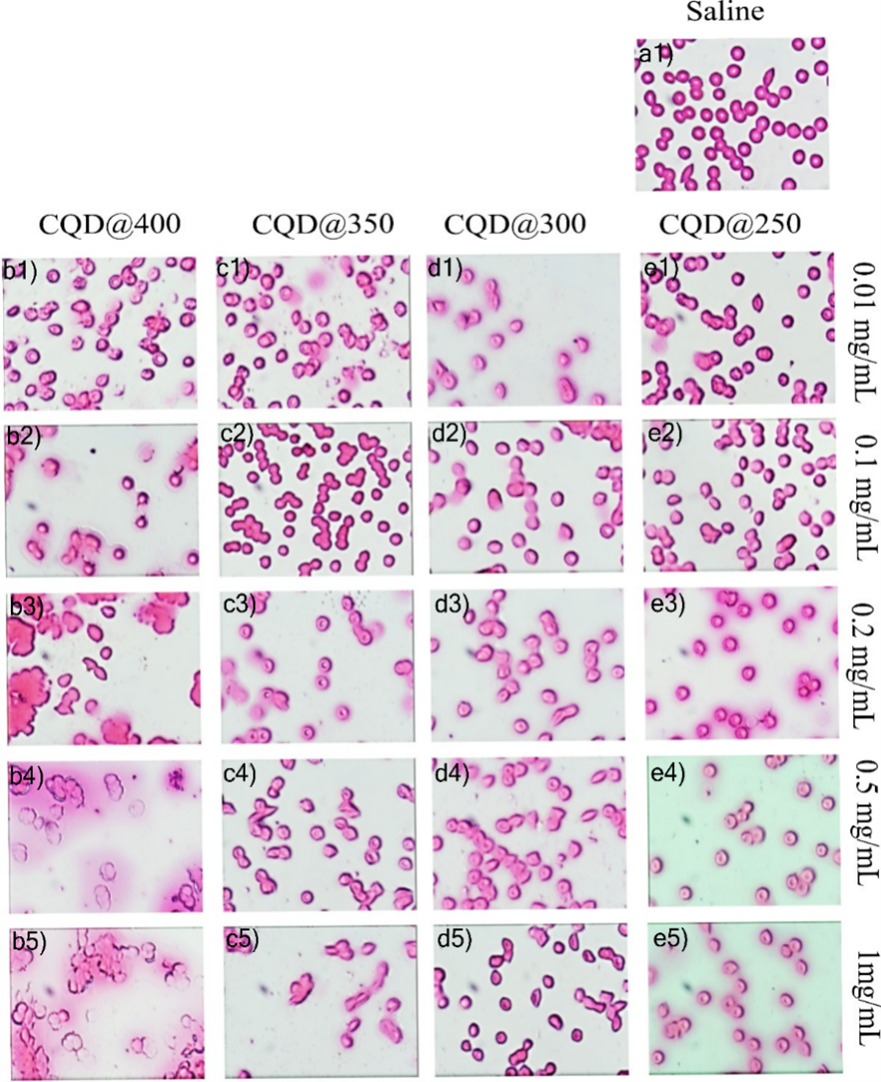
\includegraphics[width=\textwidth]{appendix_figures/Picture13.png}
  \caption[Giemsa-stained RBCs treated with CQD variants]{Pictorial representation
    of Giemsa-stained RBCs after 8\,h incubation at 37\,\textdegree C.
    \textbf{(a1)}~Control (saline).
    CQD@400: \textbf{(b1)}~0.01, \textbf{(b2)}~0.1, \textbf{(b3)}~0.2,
    \textbf{(b4)}~0.5, \textbf{(b5)}~1\,mg\,mL$^{-1}$.
    CQD@350: \textbf{(c1)--(c5)}.
    CQD@300: \textbf{(d1)--(d5)}.
    CQD@250: \textbf{(e1)--(e5)} at the same concentration series.}
  \label{fig:s11_giemsa}
\end{figure}

\begin{figure}[htbp]
  \centering
  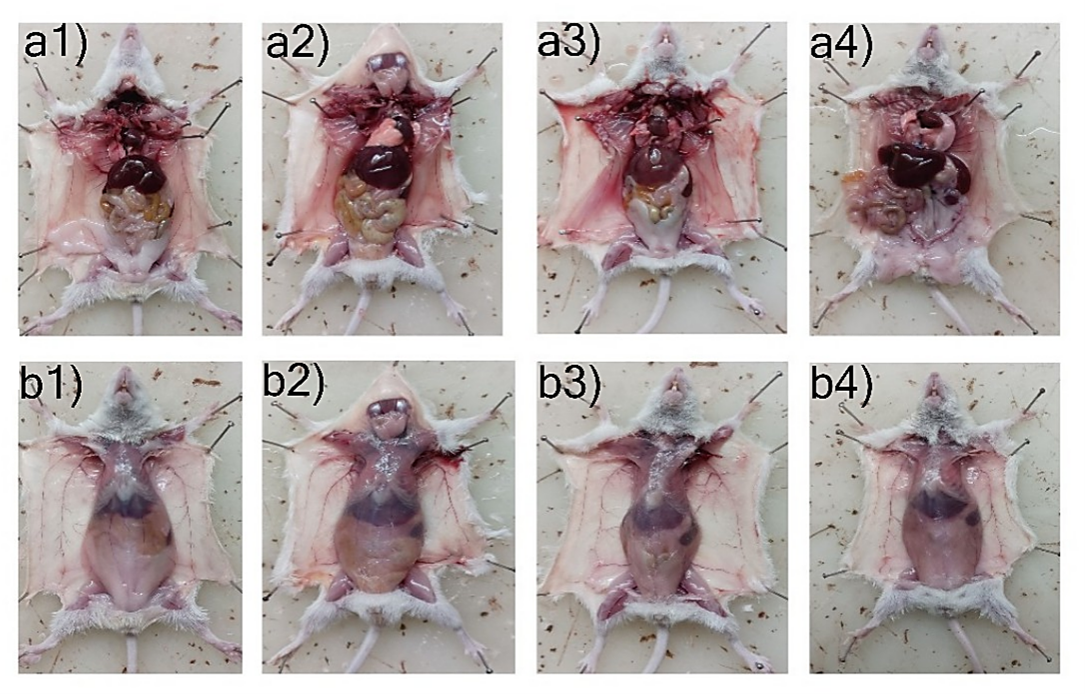
\includegraphics[width=0.90\textwidth]{appendix_figures/Picture14.png}
  \caption[Internal organ morphology after acute toxicity study]{Internal organs and
    morphology of mice observed after a 2000\,mg\,kg$^{-1}$ dose of CQD@250 following
    28 days of post-treatment observation. \textbf{(a1)--(a4)}~Internal organs of four
    different mice showing normal morphology without fluid accumulation.
    \textbf{(b1)--(b4)}~Physical appearance at the organ level, lymph node morphology,
    and peritoneal cavity without fluid accumulation for four different mice.}
  \label{fig:s12_organs}
\end{figure}

\begin{figure}[htbp]
  \centering
  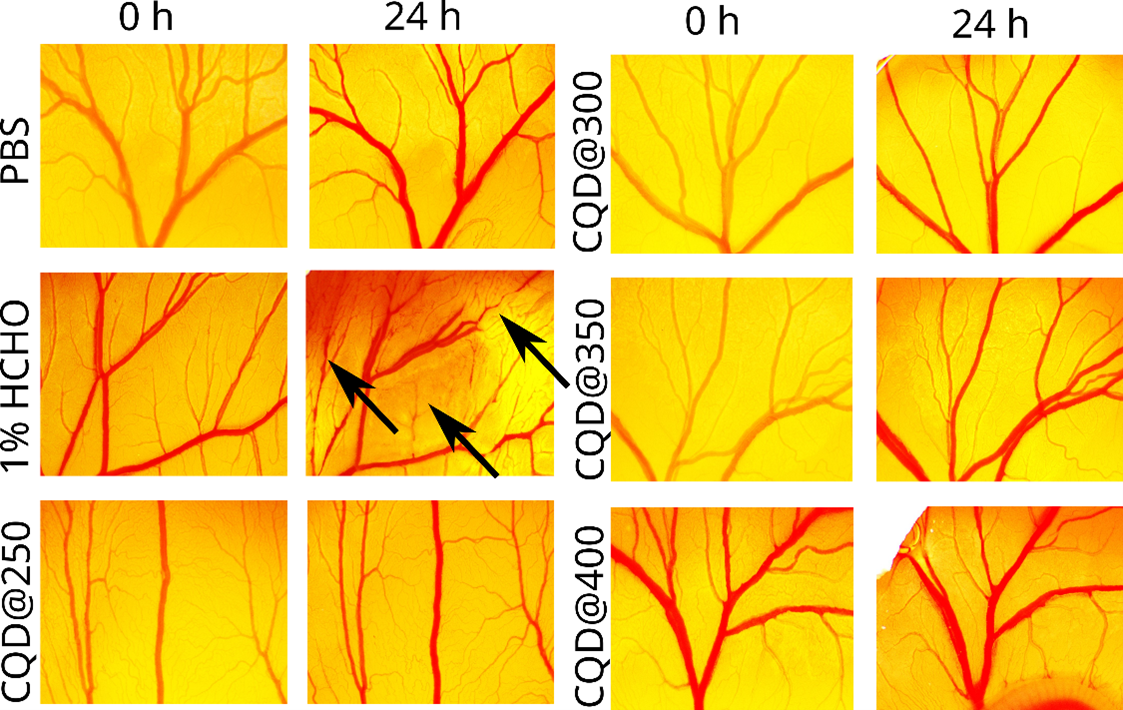
\includegraphics[width=0.80\textwidth]{appendix_figures/Picture17.png}
  \caption[Molecular docking of CQDs with ARG1 and ARG2]{Molecular docking results
    of carbon quantum dots (CQDs) with ARG1 (top) and ARG2 (bottom).
    3D representations show the active site and directly interacting chains (red
    helices); 2D interaction maps display residues and bond distances (\AA).}
  \label{fig:s13_docking}
\end{figure}

\begin{figure}[htbp]
  \centering
  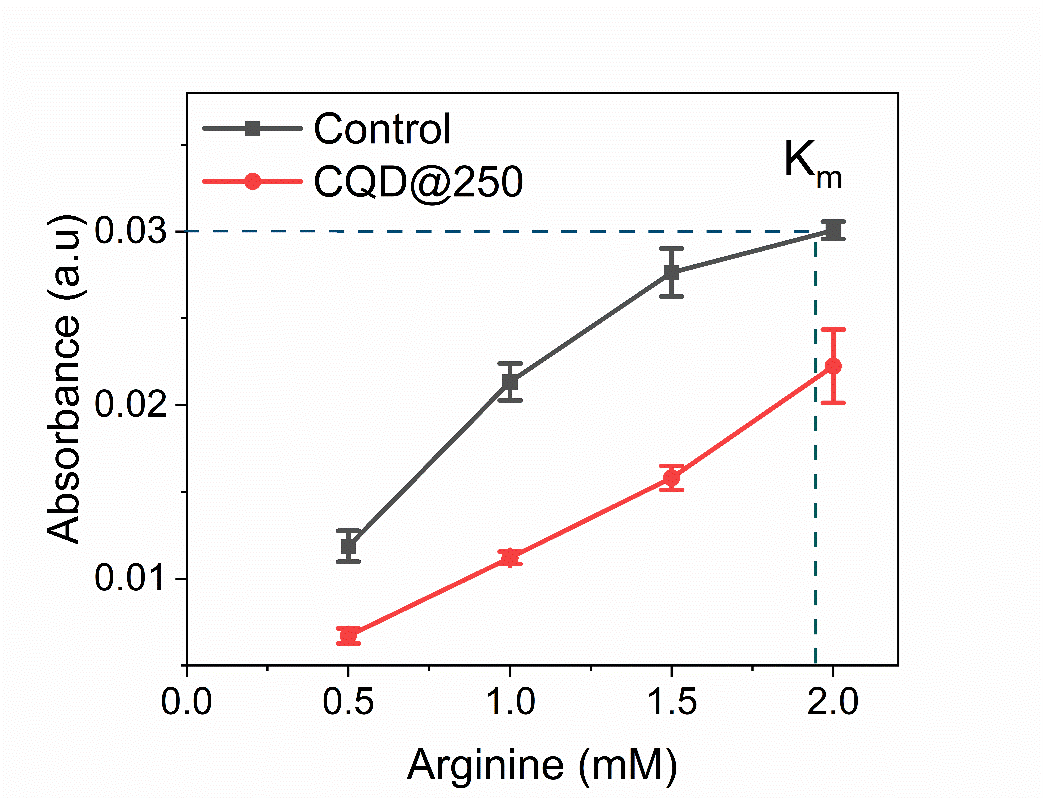
\includegraphics[width=0.60\textwidth]{appendix_figures/Picture18.png}
  \caption[Arginase inhibition kinetics -- Michaelis--Menten model]{Arginase
    inhibition in a cell-free system. Michaelis--Menten kinetics of arginase activity
    (absorbance at 520\,nm \textit{vs.}\ arginine concentration, mM) in the presence
    of CQD@250 (red) compared with control (black). The dashed line marks the $K_m$
    value of the uninhibited enzyme.}
  \label{fig:s14_mm}
\end{figure}

\begin{figure}[htbp]
  \centering
  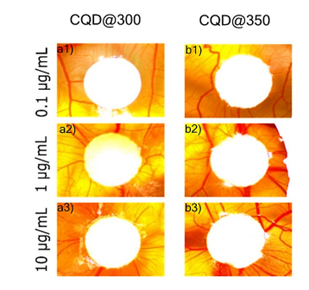
\includegraphics[width=0.70\textwidth]{appendix_figures/Picture9.png}
  \caption[YSM irritation study with CQDs]{Irritation study performed on the chick
    embryo yolk sac membrane model in the presence of CQDs (PBS negative control,
    1\% HCHO positive control, CQD@250--400 treatment groups, 0\,h and 24\,h
    time-points). Black arrows indicate sites of membrane irritation in the positive
    control (1\% HCHO) group.}
  \label{fig:s15_irritation}
\end{figure}

% ------------------------------------------------------------
\section*{Supporting Tables}
% ------------------------------------------------------------

\begin{table}[htbp]
  \centering
  \caption{Genes and proteins co-expressed with ARG1 and their associated functions.}
  \label{tab:arg1_coexpr}
  \small
  \begin{tabular}{clll}
    \hline
    \textbf{S.No.} & \textbf{Gene} & \textbf{Protein} & \textbf{Function} \\
    \hline
    1  & MDK       & Midkine (MK)                              & Growth factor \\
    2  & SDC4      & Syndecan-4                                & Cell adhesion \\
    3  & LILRB1    & Leukocyte Ig-like receptor B1             & Inhibitory cytokine receptor \\
    4  & IFNA2     & Interferon alpha-2                        & Immunomodulatory cytokine \\
    5  & IFNL1     & Interferon lambda 1                       & Antiviral cytokine \\
    6  & LILRB4    & Leukocyte Ig-like receptor B4             & Inhibitory receptor on myeloid cells \\
    7  & LILRB2    & Leukocyte Ig-like receptor B2             & Inhibitory immune receptor \\
    8  & LGALS9C   & Galectin-9C                               & Cell--cell interactions \\
    9  & IFNB1     & Interferon beta-1                         & Antiviral cytokine \\
    10 & HLA-G     & Human Leukocyte Antigen G                 & NK- and T-cell inhibitor \\
    11 & HLA-E     & Human Leukocyte Antigen E                 & NK-cell modulator \\
    12 & ANXA1     & Annexin A1                                & Leukocyte migration \\
    13 & LGALS9    & Galectin-9                                & Immune regulation \\
    14 & LGALS9B   & Galectin-9B                               & Immune regulation \\
    15 & CTSG      & Cathepsin G                               & Neutrophil protease \\
    16 & HMGB1     & High Mobility Group Box 1                 & DAMP protein \\
    17 & CD86      & CD86 (B7-2)                               & T-cell inhibition \\
    18 & PDCD1LG2  & PD-L2                                     & PD-1 ligand \\
    19 & TNFAIP8L2 & TNF$\alpha$-induced protein 8-like 2      & Immune regulation \\
    20 & CD80      & CD80 (B7-1)                               & CTLA-4 co-stimulator \\
    21 & HAVCR2    & TIM-3                                     & Immune checkpoint receptor \\
    22 & CD274     & PD-L1                                     & PD-1 ligand \\
    23 & CR1       & Complement receptor 1 (CD35)              & Complement regulation \\
    24 & CTLA4     & CTLA-4                                    & Immune checkpoint receptor \\
    25 & FOXP3     & Forkhead box P3                           & T-regulatory cell transcription factor \\
    26 & BMP4      & Bone Morphogenetic Protein 4              & Immune modulation \\
    27 & HLA-DRB1  & HLA-DR Beta 1                             & MHC class II \\
    28 & FGL1      & Fibrinogen-like Protein 1                 & T-cell suppressor \\
    29 & TWSG1     & Twisted Gastrulation BMP Modulator 1      & Immune differentiation \\
    30 & VTCN1     & B7-H4                                     & T-cell suppressor \\
    31 & LAX1      & Lymphocyte Transmembrane Adaptor 1        & TCR inhibitor \\
    32 & PTPN22    & Protein Tyrosine Phosphatase NR 22        & TCR-signalling inhibitor \\
    33 & TIGIT     & TIGIT                                     & T-cell inhibitor \\
    34 & ARG1      & Arginase 1                                & Arginase \\
    35 & VSIR      & VISTA                                     & Immune checkpoint receptor \\
    36 & VSIG4     & CRIg                                      & Complement receptor \\
    \hline
  \end{tabular}
\end{table}

\begin{table}[htbp]
  \centering
  \caption{Urine analysis of mice from acute toxicity study at a dose of
           2000\,mg\,kg$^{-1}$.}
  \label{tab:urine}
  \small
  \begin{tabular}{clllllll}
    \hline
    \textbf{S.No.} & \textbf{Parameter} & \textbf{Normal range} & \textbf{Units}
      & \textbf{Day 1} & \textbf{Day 8} & \textbf{Day 15} & \textbf{Day 28} \\
    \hline
    1  & Colour          & Clear--slightly yellow & --           & Pale yellow  & Pale yellow  & Straw        & Pale yellow \\
    2  & Transparency    & Transparent            & --           & Transparent  & Transparent  & Transparent  & Transparent \\
    3  & Leukocytes      & 10                     & cells/\textmu L & 15        & 15           & 125          & 70 \\
    4  & Nitrite         & Absent                 & --           & Absent       & Absent       & Absent       & Absent \\
    5  & Urobilinogen    & 1.68--16               & \textmu mol/L & 16          & 16           & 16           & 16 \\
    6  & Protein         & 1.52                   & g/L          & 1.0          & 1.0          & 1.0          & 0.3 \\
    7  & pH              & 5.0--5.6               & --           & 6.5          & 7.5          & 7.0          & 7.5 \\
    8  & Blood           & Absent                 & --           & $-$ve        & $-$ve        & $-$ve        & $-$ve \\
    9  & Specific gravity& 1.045--1.064           & --           & 1.030        & 1.030        & 1.015        & 1.015 \\
    10 & Ketone bodies   & 0.6                    & mmol/L       & $-$ve        & $-$ve        & 0.5          & 0.5 \\
    11 & Bilirubin       & 1.71--11.97            & \textmu mol/L & 100         & 100          & 17           & 50 \\
    12 & Glucose         & 0.033--0.1443          & mmol/L       & $>$5         & $>$5         & $>$5         & $-$ve \\
    \hline
  \end{tabular}
\end{table}

\begin{table}[htbp]
  \centering
  \caption{Physical properties of CQD@250.}
  \label{tab:cqd_props}
  \begin{tabular}{clll}
    \hline
    \textbf{S.No.} & \textbf{Property} & \textbf{Value} \\
    \hline
    1 & Density            & 2.125\,g\,cm$^{-3}$ \\
    2 & pH (10\,mg\,mL$^{-1}$) & 7.8 \\
    3 & Quantum yield      & 39.86\% \\
    4 & Fluorescence lifetime & 300\,ns \\
    \hline
  \end{tabular}
\end{table}



% ============================================================
%  Appendix: Chapter 3 – Part 1 Supporting Information
%  Protective effects of cross-linked poly-N-acryloyl glycine
%  nanoparticles in type 2 diabetes-induced complications:
%  in vivo study
% ============================================================

